\documentclass[10pt,a4paper]{amsart}
\usepackage[margin=19mm]{geometry}
\usepackage{amsmath,amssymb,mathtools}
\usepackage[scr=rsfs,cal=euler]{mathalfa}
\usepackage{xfrac}
\usepackage[unicode,hidelinks,bookmarks=false]{hyperref}
\newcommand{\ie}{i.e.\ }
\newcommand{\cf}{cf.\ }
\newcommand{\resp}{respectively\ }
\newcommand{\Subsection}{\subsection}
\providecommand{\nobreakdash}{\nobreak\hbox{-}}
\setlength{\emergencystretch}{2em}
\multlinegap0pt
\usepackage{tikz}
\usepackage{amssymb}
\newtheorem{lemma}{Lemma}
\usepackage{cleveref}
\crefname{lemma}{Lemma}{Lemmas}
\newcommand*\diff{\,\mathop{}\! \mathrm{d}\hspace*{-0.15em}\bar{}\hspace*{0.13em}}
\title{Mean Value for Random Ideal Lattices}
\author{Nihar Gargava, Maryna Viazovska}
\date{Source: arXiv:2411.14973v3 (CC BY 4.0)}
\begin{document}
\maketitle

\noindent\emph{Source and licence.} Mean Value for Random Ideal Lattices. Version arXiv:2411.14973v3 (CC BY 4.0), distributed by arXiv under the Creative Commons Attribution 4.0 International licence, http://creativecommons.org/licenses/by/4.0/, as recorded in the arXiv licence metadata for this exact version and shown on the abstract page https://arxiv.org/abs/2411.14973v3. Full licence notice: \texttt{licenses/arxiv-2411.14973-CC-BY-4.0.txt}.\par\smallskip

\noindent\textit{Editorial scope.} Counted unit: the article's lemma le:gamma\_estimate (source0.tex lines 983--990). The article's complete original proof of it is delivered with it (source0.tex lines 991--1140, one \texttt{proof} environment of 150 lines). No mathematics is written, repaired or re-derived: the statement and the proof are the article's own lines, in the article's own notation, and no retained line is substituted or re-flowed.  No further source-local context is needed: every cross-reference of every retained line resolves inside the two delivered spans.  Nothing was omitted from any retained span, so the package carries no omission record.  No retained line contains a citation, so the wrapper carries no bibliography and no bibliography entry.  The retained lines contain the article's own diagram code, which the wrapper typesets with the standard tikz packages; no image file is delivered and the package declares no asset dependency.  Editorial formatting only, in addition: an AMS \texttt{amsart} preamble that restates the article's own declarations and macros used by the retained lines, namely the environments \texttt{lemma} on separate counters, together with the standard packages those lines need.  The retained environments print in this document as Lemma 1 in order of appearance, whereas the article prints the same items with the numbering of its own full document.  The complete native source of the article as distributed in the arXiv e-print for this exact version is bundled unchanged as \texttt{sources/168953/source0.tex}.
\begin{lemma}
  \label{le:gamma_estimate}
For some constant $c_{1}>0$ which does not depend on $r_{1},r_{2}$ and $t$, we have
\begin{equation}
	\log\left| {    G(\tfrac{1}{2} + i t) }\right|  
    \leq  - \left(\tfrac{1}{4} d \log d - c_{1} d \right)  - \tfrac{r_{1}+r_{2}-1}{4}\log\left( t^{2} + \tfrac{1}{4}\right)
\end{equation}
\end{lemma}

\begin{proof}

We begin with the exact Stirling approximation formula. For $|\arg(s)|< \pi - \varepsilon$, where $\varepsilon > 0$, it states
\begin{equation}
	\label{eq:stirling}
    \log  \Gamma(s) =  \left( s- \tfrac{1}{2}\right)   \log s - s + \tfrac{1}{2}\log (2 \pi) + E(s)
\end{equation}
where 
\begin{equation}
    E(s) = \int_{0}^{\infty} \frac{ 2\arctan(\frac{x}{s})}{e^{2 \pi x} - 1} \diff x.
\end{equation}

Our main interest is in estimating for $s= 1/2+it$
\begin{equation}
    \Delta(s) =  \Re( r_{1}E(s/2) + r_{2} E(s) - E(ds/2)),
\end{equation}
since the real part alone contributes to the absolute value of $G(s)$.




We know that 
\begin{equation}
\arctan s =  \frac{1}{2i} \log\left( \frac{1 + is}{ 1 - is}\right).
\end{equation}

Therefore, when $s = \sigma + it$ for $\sigma>0$, one has 
\begin{equation}
2 \Re(\arctan (x/s)) = 
\arg \left( \frac{\sigma + i(t+x)}{\sigma + i (t-x)} \right) 
= 
\arg \left( \frac{1 + i(t+x)\sigma^{-1}}{1 + i (t-x)\sigma^{-1}} \right) 
.
\end{equation}

Denote 
\begin{equation}
    a(x,t) = \arg\left(  \frac{1 + i(t+x)}{ 1 + i(t-x)} \right).
\end{equation}
This function therefore measures the angle subtended from the origin by a segment of length $2x$ between $1+i(t+x)$ and $1-i(t-x)$.
See~\cref{fig:angle}.

\begin{figure}
    \centering


\tikzset{every picture/.style={line width=0.75pt}} %set default line width to 0.75pt        

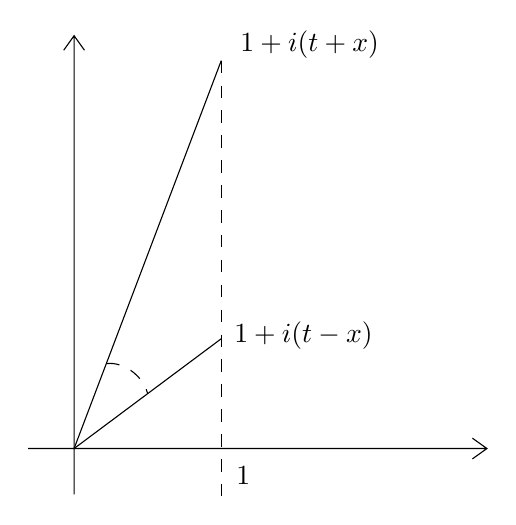
\begin{tikzpicture}[x=0.75pt,y=0.75pt,yscale=-1,xscale=1]

\draw  (17,233.9) -- (238,233.9)(39.1,35) -- (39.1,256) (231,228.9) -- (238,233.9) -- (231,238.9) (34.1,42) -- (39.1,35) -- (44.1,42)  ;
\draw  [dash pattern={on 4.5pt off 4.5pt}]  (110,47) -- (110,257) ;
\draw    (110,47) -- (39.1,233.9) ;
\draw    (110,181) -- (39.1,233.9) ;
\draw  [dash pattern={on 4.5pt off 4.5pt}]  (55,193) .. controls (62,192) and (72,198) .. (74.55,207.45) ;

\draw (122,148) node [anchor=north west][inner sep=0.75pt]   [align=left] {};
\draw (115,171.4) node [anchor=north west][inner sep=0.75pt]    {$1+i( t-x)$};
\draw (116,241.4) node [anchor=north west][inner sep=0.75pt]    {$1$};
\draw (118,31.4) node [anchor=north west][inner sep=0.75pt]    {$1+i( t+x)$};

\end{tikzpicture}

\caption{ The function $a(x,t)$ measures for $x>0$ the angle subtended at the origin. One can argue from this picture that $a(4x,2t) \geq a(2x,2t)$ for every $t \in \mathbb{R}$ and $x>0$.}
\label{fig:angle}
\end{figure}

Then, we have an expression for $\Delta(\frac{1}{2} + it)$  as
\begin{align}
	\Delta(\tfrac{1}{2}+it) 
	& =  \int_{0}^{\infty} \frac{r_{1}a(4x,2t) + r_{2} a(2x,2t) - a(\tfrac{4}{d} x, 2t) }{ e^{2 \pi x} - 1} dx \\
\end{align}

Observe that one has $a(4x,2t) \geq a(2x,2t)$ because the angle subtended is larger. Hence, we write
\begin{equation}
    \Delta\left(\tfrac{1}{2}+it\right) \leq 
    (r_{1}+r_{2}) 
    \int_{0}^{\infty}  \frac{a(4x,2t)}{e^{2 \pi x} - 1} \diff x
\end{equation}.

For $x \geq 0$, we estimate
\begin{equation}
    a(x,t) \leq 
    \begin{cases}
	\frac{2x}{1+t^{2} - x^{2}} & \text{ when } 
\frac{2x}{1+t^{2} - x^{2}}  \leq \pi \\
	\pi & \text{ otherwise }
    \end{cases}.
\end{equation}

The first inequality is just using that $\arctan x\leq x$ for positive $x$ and the second uses that $\arctan x \leq \pi/2$ for large values. We observe that for $x > 0$ one has 
\begin{equation}
x \leq -\frac{1}{\pi} + \sqrt{1+t^{2} + \frac{1}{\pi^{2}}}  \Leftrightarrow  \frac{2x}{1+t^{2}-x^{2}} \leq \pi
\end{equation}

Denote $$c(t) = -1/\pi + \sqrt{1 + t^{2} + 1/ \pi^{2} }.$$
Then, one estimates that 
\begin{equation}
   \frac{1}{r_{1}+r_{2}} \Delta\left(\frac{1}{2}+it\right) 
    \leq 
 \int_{0}^{ \tfrac{1}{4}c(2 t) } \frac{ (e^{2\pi x} -1)^{-1} 8x}{1+4 t^{2}-16 x^{2}} \diff x  +  \int_{\tfrac{1}{4}c(2t)}^{\infty} \frac{\pi}{ e^{2 \pi x} - 1} \diff x
\end{equation}

We estimate that $e^{2\pi x} - 1 \geq x$ for positive $x$. The first integral is then exactly solvable and we can estimate it as 
\begin{equation}
    \leq C \frac{ \ln( 2 + |t|)}{\sqrt{1+t^{2}}} \text{ for some }  C>0
\end{equation}
 and for the second we observe that $c(t) \geq C_1$ for some constant $C_{1} > 0$ therefore we can assume $(e^{2\pi x} - 1)^{-1} \leq C_{2} e^{-2 \pi x}$ for some $C_2$. Hence the second we get a bound of
\begin{equation}
    \leq C_{3} e^{-C_{4} t} \text{  for some  } C_{3},C_{4} > 0.
\end{equation}

Combined, this gives us that for all values of $r_{1},r_{2}$
\begin{equation}
    \Delta(\tfrac{1}{2}+it) \leq  (r_{1}+r_{2}) \tfrac{c \ln(2 + |t|)}{\sqrt{1+t^{2}}} \text{ for some } c>0.
\end{equation}
For our use, we can completely ignore the dependence on $t$ and write that 
\begin{equation}
    \Delta(\tfrac{1}{2}+it) \leq  (r_{1}+r_{2}) {c}\text{ for some } c>0.
\end{equation}


By using Stirling's approximation from~\cref{eq:stirling}, we get 
\begin{align}
    & \log |G(s)| 
    =  \Re( \log G(s)) \\
    % =  \Re \Big(  \tfrac{s-1}{2} \log s  - \tfrac{1}{2}s + \Big) \\
    = & \left( r_{1} \Re(\tfrac{s}{2} \log {s}) -   \tfrac{r_{1}}{2}(\log 2)\Re({s} )  \right) 
    + r_{2} \Re (s \log s) 
    - \left(\tfrac{d}{2} \Re(s \log s) + \tfrac{d}{2} (\log \tfrac{d}{2})\Re(s )  \right) \\ 
      & - \left(\tfrac{r_{1}+r_{2}-1}{2}\right) \Re(\log s) 
      + \tfrac{r_{1}}{2} \log 2 +  \tfrac{1}{2}\log (\tfrac{d}{2})  + \tfrac{r_{1}+r_{2} - 1 }{2} \log (2 \pi) 
      -(r_{1}+r_{2}-1)\Re(s)
 +
      \Delta(s) .
\end{align}
The terms involving $\Re(s \log s)$ cancel out.
We use the fact that $\Re(s) = 1/2$ which gives us $\Re(\log (s)) = \tfrac{1}{2}\log (t^{2} + 1/4)$. 
Then, using our estimate above
we get that 
\begin{align}
     \log |G(s)|  
     % \leq &   - \tfrac{1}{4} d \log d - \tfrac{r_{1}+r_{2}-1}{4} \log (t^{2} + \tfrac{1}{4}) 
     % + r_{1} \Big(\tfrac{\log 2}{ 4} + \tfrac{\log (2\pi)}{2} - \tfrac{1}{2}\Big) \\
     %   & + r_{2} \Big( \tfrac{ \log (2\pi)}{ 2} - \tfrac{1}{2}\Big) + \tfrac{1}{2} \log ( \tfrac{d}{2}) + c \\ 
     \leq &   
     \left( -\tfrac{1}{4} d \log d + c_{1} d \right)  - \tfrac{r_{1}+r_{2}-1}{4}\log\left( t^{2} + \tfrac{1}{4}\right),
\end{align}
where $c,c_{1} > 0$ are some constants.
\end{proof}

\end{document}
